\documentclass[12pt,fleqn]{article}\usepackage{../common}
\begin{document}
Lineer Cebir - Ders 3

Onceki derslerde matris carpimi yaptik, bu derste bu islemin kurallarini
gorecegiz. Bu isi pek cok sekilde yapmanin yolu var ve hepsi onemli, ve
ayni sonucu veriyor.

Sonra matris tersi (inverse) konusuna girecegiz, orada bir suru kavram var,
ve cok onemli. 

Iki matrisi carpma teknigiyle baslayalim. 

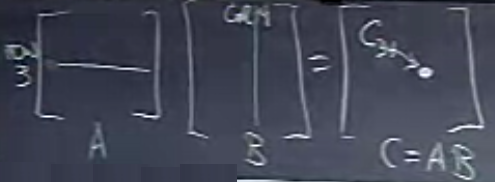
\includegraphics[height=4cm]{3_01.png}

Bu carpimi yaparken soldaki matrisin uzerinde sol isaret parmagi,
sagdakinde sag isaret parmagi konulur, ve soldan-saga, yukaridan-asagi iki
el hareket ettirilir, ve gosterilen hucreler birbiri ile carpilir, bu
carpimlar toplanir. Ustte soldaki matrisin 3. satiri, sagdaki matrisin
4. kolonu baz alinmis, bu carpim ve toplama sonucu $C$'nin 3. satir ve
4. kolonundaki degeri elde ederiz. Bu degere $c_{34}$ diyelim,

$$ 
\left[\begin{array}{rrrr}
\\
\\
a_{31} & a_{32} & \dots \\
\\
\\
\end{array}\right]
\left[\begin{array}{rrrrr}
& & b_{14} & & \\
& & b_{24} & & \\
& &  & & \\
& &  & & \\
& &  & & 
\end{array}\right] 
=
\left[\begin{array}{rrrrr}
& &  & & \\
& &  & & \\
& & c_{34} & & \\
& &  & & \\
& &  & & 
\end{array}\right]
$$

$$ c_{34} = \textrm{ 3. satir } \times \textrm{ 4. kolon } $$

$$ = a_{31}b_{14} + a_{32}b_{24} + ... $$

Eger toplama operatorunu kullanarak daha temiz yazmak gerekirse,

$$ c_{34} = \sum_{k=1}^{n} a_{3k}b_{k4} $$
ki $n$ satir sayisi $n$'dir. 

Bu carpimi tabii her zaman gerceklestiremeyiz. Carpimin olmasi icin matris
boyutlarinin uyumlu olmasi gerekir (illa kare matris olmalari
gerekmez). Ustteki carpimin nasil gerceklestigine bakarsak bu uyumu gormeye
baslariz herhalde, soldaki matrisin satiri sagdakinin kolonu carpiliyorsa
bu satir ve kolon buyukluklerinin esit olmasi gerekir. Diyelim ki $m$ satir
$n$ kolon iceren $A$ matrisi $m \times n$ boyutlarinda ise, o zaman bu
matris sadece $n \times p$ boyutlarindaki bir $B$ matrisi ile
carpilabilir, ve sonuc $m \times p$ boyutlarinda yeni bir matris olur. 

Bu matris carpimina kolon bazli bakabilir miyiz? Evet. Daha once
ogrendigimiz kolon carpi matris fikrini kullanmak yeterli, mesela alttaki
durumda

$$ 
\underbrace{
\left[\begin{array}{rr}
\dots & \dots   \\
\dots & \dots   \\
\dots & \dots 
\end{array}\right]
}_{A m \times n}
\underbrace{
\left[\begin{array}{rr}
\uparrow &  \dots\\
&  \dots\\
\downarrow & \dots 
\end{array}\right] 
}_{B, n \times p}
=
\underbrace{
\left[\begin{array}{rr}
\uparrow &  \dots \\
&  \dots \\
\downarrow & \dots
\end{array}\right] 
}_{C, m \times p}
$$

$A$'nin {\em tamaminin} $B$'nin en sol kolonu ile carpilmasi bize $C$'nin
en sol kolonunu verir. Dikkat, bu islemde $B$'nin diger kolonlari hicbir
sekilde isleme dahil olmazlar. Eger yine $A$'nin {\em tamami} ile bu sefer
ikinci kolonu carparsak $C$'nin ikinci kolonunu elde ederiz, vs.

$$ 
\underbrace{
\left[\begin{array}{rr}
\dots & \dots   \\
\dots & \dots   \\
\dots & \dots 
\end{array}\right]
}_{A m \times n}
\underbrace{
\left[\begin{array}{rr}
\dots & \uparrow \\
& \\
\dots & \downarrow
\end{array}\right] 
}_{B, n \times p}
=
\underbrace{
\left[\begin{array}{rr}
\dots & \uparrow \\
& \\
\dots & \downarrow
\end{array}\right] 
}_{C, m \times p}
$$

O zaman su ifadeyi kullanabiliriz: ``$C$'nin her kolonu $A$'nin
kolonlarinin bir kombinasyonudur''. Bu ifade daha onceki kolon bakisimiz
ile uyumlu. Daha once kolonlarin kombine edilerek yeni bir kolon elde
edildigini gorduk, bu fikri sadece $B$ uzerinde, tekrar tekrar, her kolon
icin ayri ayri uyguluyoruz, ve sonuc olarak $C$'nin ayri ayri kolonlarini
elde ediyoruz.

Satir Bakisi

$$ 
\underbrace{
\left[\begin{array}{rr}
\leftarrow  & \rightarrow  \\
\dots & \dots \\
\dots & \dots 
\end{array}\right]
}_{A m \times n}
\underbrace{
\left[\begin{array}{rr}
\dots & \dots \\
\dots & \dots \\
\dots & \dots
\end{array}\right] 
}_{B, n \times p}
=
\underbrace{
\left[\begin{array}{rr}
\leftarrow  & \rightarrow  \\
\dots & \dots  \\
\dots & \dots 
\end{array}\right] 
}_{C, m \times p}
$$

Ayni carpimi satirsal olarak dusunelim, tekrar daha once ogrendigimiz satir
bakisini ayri ayri satirlar olarak kullaniyoruz. $A$'nin tek bir satiri
$B$'nin tamamini, tum satirlarini kombine ediyor ve bu sekilde $C$'nin
tekabul eden satirini elde ediyoruz. 












\end{document}
